\documentclass[tikz,border=2pt]{standalone}
\usepackage{amsmath}
\usetikzlibrary{arrows.meta}
\begin{document}
% One lifetime with death in (K_x, K_x+1): the annuity-due Y pays at 0,...,K_x, the annuity-immediate Y*
% at 1,...,K_x, so Y* = Y - 1 (only the certain time-0 payment is dropped). Shifting Y by one year (vY)
% would pay at 1,...,K_x+1, including a payment after death: a_x is not v times the annuity-due APV.
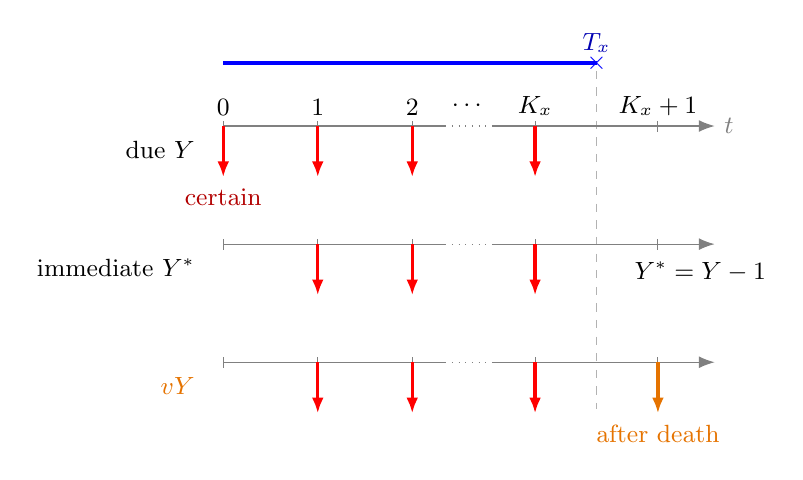
\begin{tikzpicture}[font=\small, >={Latex[length=2mm]}, x=1.2cm]
  \newcommand{\taxis}[1]{%
    \draw[gray] (0,#1) -- (2.35,#1);
    \draw[gray, dotted] (2.35,#1) -- (2.85,#1);
    \draw[gray, ->] (2.85,#1) -- (5.2,#1);
    \foreach \t in {0,1,2,3.3,4.6} \draw[gray] (\t,#1-0.07) -- (\t,#1+0.07);}
  % time labels and the life
  \foreach \t/\l in {0/0,1/1,2/2,3.3/K_x,4.6/K_x+1} \node[above, inner sep=2pt] at (\t,0.05) {$\l$};
  \node at (2.6,0.25) {$\cdots$};
  \node[gray, anchor=west] at (5.2,0) {$t$};
  \draw[blue, very thick] (0,0.8) -- (3.95,0.8);
  \node[blue] at (3.95,0.8) {$\times$};
  \node[blue!70!black, above, inner sep=2pt] at (3.95,0.85) {$T_x$};
  \draw[gray!60, thin, dashed] (3.95,0.7) -- (3.95,-3.6);
  % annuity-due
  \taxis{0}
  \node[anchor=east] at (-0.2,-0.3) {due $Y$};
  \foreach \t in {0,1,2,3.3} \draw[red, very thick, ->] (\t,0) -- (\t,-0.65);
  \node[red!70!black, anchor=north] at (0,-0.68) {certain};
  % annuity-immediate
  \taxis{-1.5}
  \node[anchor=east] at (-0.2,-1.8) {immediate $Y^*$};
  \foreach \t in {1,2,3.3} \draw[red, very thick, ->] (\t,-1.5) -- (\t,-2.15);
  \node[anchor=west] at (4.25,-1.85) {$Y^*=Y-1$};
  % one-year shift of the annuity-due
  \taxis{-3.0}
  \node[orange!90!black, anchor=east] at (-0.2,-3.3) {$vY$};
  \foreach \t in {1,2,3.3} \draw[red, very thick, ->] (\t,-3.0) -- (\t,-3.65);
  \draw[orange!90!black, very thick, ->] (4.6,-3.0) -- (4.6,-3.65);
  \node[orange!90!black, anchor=north] at (4.6,-3.68) {after death};
\end{tikzpicture}
\end{document}
